\section{Problem Statement \& Motivation} \label{sec:problem-statement-motivation}

Identifying relevant research papers is an ongoing and time-consuming task for academics. This challenge is particularly pronounced for those new to a field, as they must familiarize themselves with its current research landscape. However, even seasoned researchers encounter difficulties in staying updated with the latest findings due to the rapidly increasing volume of publications. Various sources indicate that between 2.5 million \cite{WareSTMReport2015} and 3 million \cite{KhadkaCapturingExploiting2020} new research papers are published each year. Khabsa et al.'s 2014 study \cite{KhabsaNumberScholarly2014} suggests there are nearly 25 million research papers available online, with an annual growth rate ranging from $4\%$ \cite{KhadkaCapturingExploiting2020} to as high as $9\%$ \cite{BornmannGrowthRates2014}. This substantial growth complicates the task of pinpointing relevant articles.

To mitigate this issue, recommender systems have been developed to suggest pertinent papers to scholars. Yet, many researchers still gravitate towards manual search techniques, such as keyword search in digital libraries, traversing paper citation graphs, ranking papers by non-personalized metrics like citation count or recency, and even relying on recommendations from colleagues.
The subsequent sections detail the shortcomings of traditional approaches to academic paper search, underscoring the need for a more effective solution.


\subsubsection*{Search Engines}

Search engines are a popular method to find research papers. In this approach, keywords provided by the user are matched to papers in the search engine's database.
General-purpose search engines like Google\footnote{\url{https://www.google.com/}} or Bing\footnote{\url{https://www.bing.com/}} offer several advantages: they are fast, widely accessible, user-friendly, free, and multilingual. However, they aren't tailored for academic paper searches, leading to a mix of academic and non-academic content in the results. Furthermore, users lack control over the presentation order of search results and less popular papers often remain unlisted.

Specialized academic search engines like Google Scholar\footnote{\url{https://scholar.google.com/}}, Semantic Scholar\footnote{\url{https://www.semanticscholar.org/}}, IEEE Xplore\footnote{\url{https://ieeexplore.ieee.org/}}, and ACM Digital Library\footnote{\url{https://dl.acm.org/}} cater more to researchers' needs. They index only academic papers and offer enhanced search capabilities, such as filters for publication date, author, or venue. Yet, even these engines have shortcomings. Their ranking customization options are limited. For instance, Google Scholar primarily offers broad categories like \emph{date} and \emph{relevance}. Although Semantic Scholar provides a more granular set of filters and sorting options, including \emph{citation count} and \emph{most influential}, the mechanics of their ranking algorithms including the features that impact the relevance metric remain opaque.

Additionally, these platforms typically present rankings without a quantifiable relevance score, preventing users from gauging the relative pertinence of papers or determining how closely search results align with their queries in absolute terms.

\subsubsection*{Following Citations}

Another strategy for identifying relevant papers is to trace the citations of a paper that the user considers valuable. This method is based on the premise that papers that cite each other are thematically connected.
\Cref{fig:following-citations} depicts this process with an example. The referenced paragraph contains links to two other citations, suggesting that the cited papers are related to the citing paper's topic and might be of interest to the reader.

\begin{figure}[htb!]
    \centering
    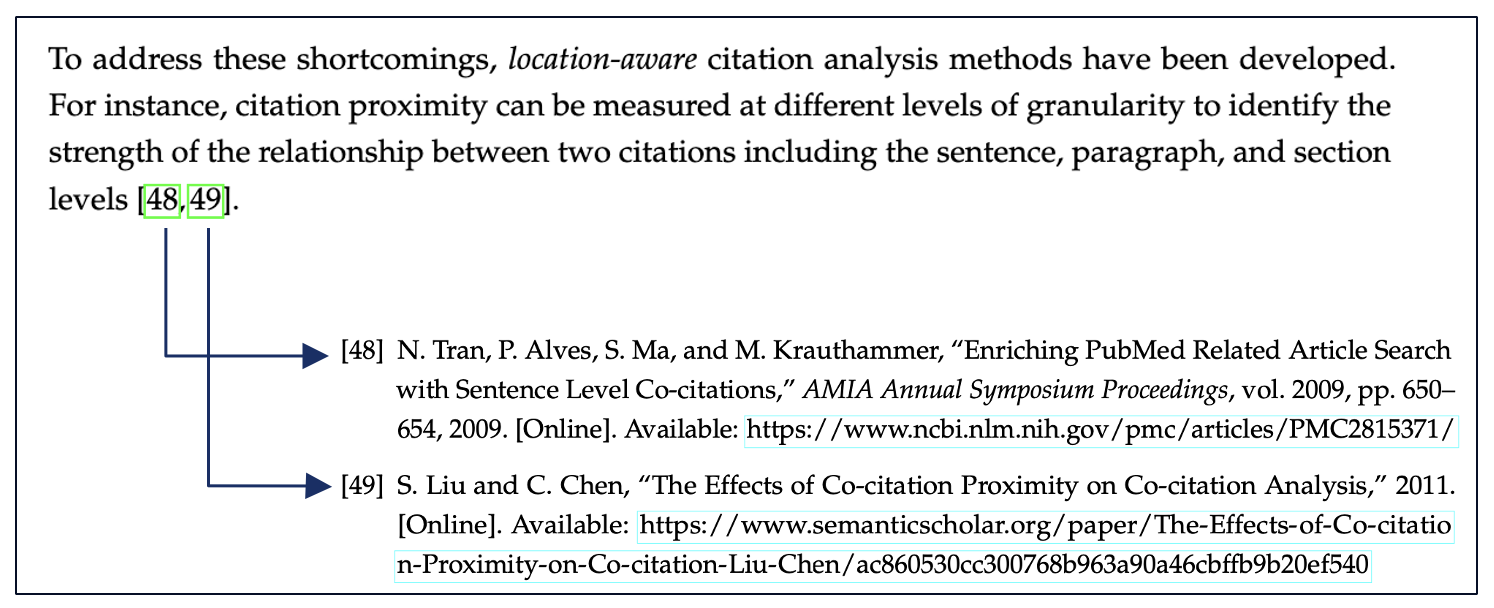
\includegraphics[width=0.9\textwidth]{screenshots/following_citations.png}
    \caption[Following Citations]{Following citations of one paper to find related papers. The cited papers are assumed to be related to the topic of the original paper and might therefore be relevant recommendations for further reading. The citation context provides clues about the scope and relevance of the cited papers.}
    \label{fig:following-citations}
\end{figure}

Navigating the citation graph offers several advantages over search engines. It's a straightforward, intuitive method and personalizes recommendations based on the user's existing interests. Moreover, the citation context provides clues about the scope and relevance of the cited papers.

Yet, this approach is not without drawbacks.
First, it is time-intensive, as users must manually select citations, evaluate their relevance, and acquire access to the cited papers.
Second, it necessitates a starting point, implying users must already be somewhat familiar with the research area.
Third, it is not scalable, as users can only follow a limited number of citations before losing track of the original paper's topic.
Fourth, the technique does not guarantee comprehensive coverage of the research landscape and relevant papers might be missed.
Finally, users strongly depend on the authors' citation practices, as they might omit relevant citations or include citations that are not thematically related to the paper.


\subsubsection*{AI Tools}

With OpenAI's launch of ChatGPT in November 2022\footnote{\url{https://openai.com/blog/chatgpt}}, several AI tools emerged that are capable of recommending research papers. Built upon \ac{LLMs} like GPT-3 \cite{BrownLanguageModels2020} or GPT-4 \cite{OpenAIGPT4Technical2023}, they offer a chat interface, allowing users to query the model in natural language.
In theory, these chatbots can offer highly tailored recommendations, letting users articulate their preferences and iteratively refine results.
Further, the model can provide immediate context to each suggestion, such as a paper summary.

Despite their potential, AI-based recommendation systems have significant limitations.
Their primary issue is reliability - recommendations are not reproducible, users have no control over the model's responses, and there is a risk of missing relevant papers.
Furthermore, without web access, these tools can only recommend papers up to their last training data update, potentially leading to outdated suggestions. Lastly, many current offerings are proprietary to some extent and might require a paid subscription to access their full functionality.


\subsubsection*{Replicating Research Approaches}

An alternate approach to finding relevant papers is to emulate research methodologies from the academic literature.
This involves studying papers on existing recommender systems, pinpointing approaches suitable for the user's domain, and replicating the described methodologies.

This method combines the advantages and disadvantages of prior strategies.
Recommendations are personalized, as researchers choose techniques aligned with their objectives.
The ranking algorithm is transparent, given that methodologies are often thoroughly outlined in the paper.
Finally, interacting with the latest research in the field gives insight into state-of-the-art recommendation techniques that might provide more accurate recommendations than solutions accessible to a broader audience.

However, this approach also poses challenges.
First, reading and understanding the papers demand a significant time investment, while replicating the methodologies - including model training - often require substantial, or even infeasible, computational resources.
Second, proposed techniques might be inaccessible to readers if the code or data is not public, if the paper omits crucial implementation details, or if the method is tailored for a specific scenario and cannot be generalized.


\subsubsection*{Shortage of Hybrid Paper Recommenders}

Much of the current research on paper recommendation focuses on singular techniques, such as either citation-based or content-based methods, and lacks the flexibility to combine different approaches.

Citation-based methods \cite{GippSciensteinResearch2009,SugiyamaExploitingPotential2013,HabibSectionsbasedBibliographic2019,GippCitationProximity2009,KnothCanWe2017} rely on the citation network to determine a paper's importance.
Such methods provide insights into a paper's perceived relevance within its community. However, a limitation of this approach is its potential bias towards well-cited papers. This can lead to overlooking newer or less cited research that might offer innovative perspectives. This bias indicates that relying solely on citation metrics can miss out on recognizing emerging areas of study.

Conversely, content-based methods \cite{MassAdhocDocument2020,CohanSPECTERDocumentlevel2020,A.MohamedBERTELMo2019,BhagavatulaContentBasedCitation2018,AgarwalResearchPaper2005,NascimentoSourceIndependent2011} focus on the textual content of documents to determine their relevance.
These systems align recommendations with distinct research themes.
However, like citation-based techniques, they pose challenges. A primary concern is their tendency to offer a narrow spectrum of recommendations.
While adept at identifying papers that match a user's specific query, they might overlook related works from other disciplines that could provide valuable insights or additional context.

Considering these strengths and shortcomings, there's a compelling case for hybrid recommender systems that synergize citation-based and content-based approaches.


\subsubsection*{Contribution of this Thesis}

This thesis presents a hybrid recommender system designed for Computer Science research that seeks to address many limitations of existing systems.
Available as free open-source software with an easy-to-use interface and detailed documentation, the system delivers automated and reproducible recommendations with transparent ranking criteria.
The hybrid structure combines global document characteristics, such as popularity and recency, with both citation and content-driven methods. It offers users the flexibility to adjust the influence of each method for customized recommendations. Additionally, the system enriches rankings with a relevance score, offering researchers insights into the relative importance of each recommendation.
